\documentclass{beamer}
\usetheme{Antibes}
\usecolortheme{whale}
\title{Human-Robot Collaboration: A Survey} 
\author{Gao Lu\inst{1} \and Tan Meng\inst{1} \and Xu Jialin\inst{1} \\ Zhan Yuxin\inst{1} \and Zhang Ziye\inst{1}}
\institute{\inst{1}School of Future Technology, Huazhong University of Science and Technology}
\date{\today}

\usepackage{tikz}
\usetikzlibrary{arrows, positioning, shadows, math}
\usepackage{xeCJK}
\usepackage{xcolor}
\usepackage{colortbl}
\usepackage{caption}
\captionsetup[figure]{labelformat=simple, labelsep=period, name=Fig, font=tiny}
\usepackage[numbers, sort&compress, super]{natbib}
\usepackage{ragged2e}

\AtBeginSection[] {
\begin{frame}
\tableofcontents[currentsection, hideothersubsections]
\end{frame}
}

\setmainfont{Noto Serif}
\setCJKsansfont{Noto Sans CJK SC}

\newcounter{industry}

\definecolor{KeyBlue}{RGB}{28, 99, 216}
\definecolor{Blue1}{RGB}{138, 175, 235}
\definecolor{Blue2}{RGB}{196, 214, 245}

\setbeamertemplate{footline}{
\leavevmode%
\hbox{
\begin{beamercolorbox}[wd=0.1\paperwidth,ht=2.25ex,dp=1mm,right]{}
\scriptsize\insertframenumber{} / \inserttotalframenumber
\end{beamercolorbox}}}

\begin{document}

\begin{frame}
\titlepage
\begin{tikzpicture}[remember picture, overlay]
\node[anchor=south east, xshift=0mm, yshift=0mm, opacity=0.2] at (current page.south east)
{
\includegraphics[width=0.25\textwidth]{sft_logo.png}};
\end{tikzpicture}
\end{frame}

\begin{frame}{Outline}
\tableofcontents[hideallsubsections]
\end{frame}

\section{Background}

\subsection{A Journey of HRC Momentum}
\begin{frame}{A Journey of HRC Momentum \cite{journey_hrc_momentum}}
\begin{itemize}
\item 1980s-2010s: Early interest from HRI \cite{An1989TheRO, 762539, 1087787, 760350, 6936985, DESANTIS2008253}
\vspace{10mm}
\item 2010s-2020s: Industrial prototype period \cite{MALIK2019665, Arash2017, GUIOCHET201743, 8107677, 9302892}
\vspace{10mm}
\item 2020s-Present: Intelligent collaboration \cite{Ji2024}
\end{itemize}
\end{frame}

\subsection{Intelligent Collaboration}
\begin{frame}{Intelligent Collaboration \cite{Ji2024}}

\begin{columns}[onlytextwidth]

\begin{column}{0.5\textwidth}
\centering
\large
Key Power of ML
\footnotesize
\vspace{2mm}
\begin{itemize}
\item Data \cite{naturestatistical, paul2023deeplearningdatadiet, karla2024data}
\vspace{5mm}
\item Algorithm \cite{Blum1998, 7724478, bp}
\vspace{5mm}
\item Computation \cite{kaplan2020scalinglawsneurallanguage}
\end{itemize}
\end{column}

\begin{column}{0.5\textwidth}
\centering
\large
Rising Road of IC
\footnotesize
\vspace{2mm}
\begin{itemize}
\item VLM Semantic Information \cite{radford2021learningtransferablevisualmodels, ravi2024sam2segmentimages}
\vspace{5mm}
\item Robot API Design \cite{vemprala2023gridplatformgeneralrobot, ros}
\vspace{5mm}
\item LLM Task Reasoner \cite{Lin2023, driess2023palmeembodiedmultimodallanguage}
\end{itemize}
\end{column}

\end{columns}
\end{frame}

\section{Case Studies}

\subsection{Industry}

\begin{frame}{工业协作机器人}

\setlength{\leftmargini}{0mm}
\begin{itemize}
\scriptsize{
\item \textbf{特征:}使人和机器人作为合作者在\textcolor{red}{同一工作空间}中并肩工作完成任务
\item \textbf{分工:}人执行需要灵巧或决策的任务部分
\newline\phantom{\textbf{分工:}}机器人实现例如重复、高负载和精确放置等工作
\item \textbf{优势:}更高的生产力和效率、更大的灵活性
}\end{itemize}

\begin{columns}[c]
\begin{column}{0.7\textwidth}
\centering
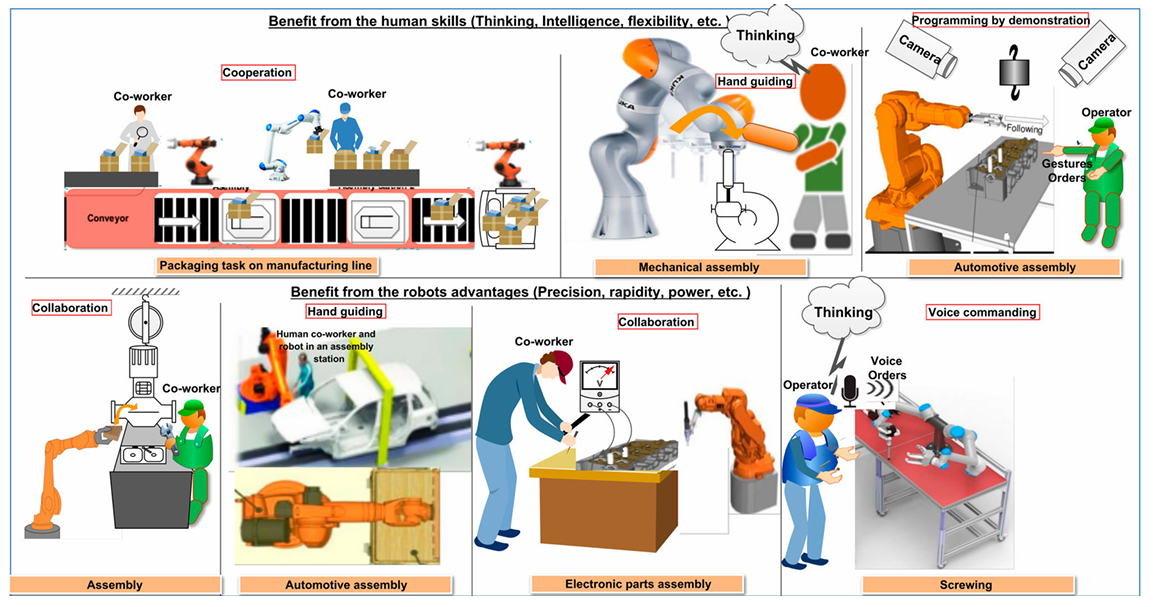
\includegraphics[width=\linewidth]{industry/1.png}
\tiny{\captionof{figure}{Human-robot collaboration examples \cite{Hentout18082019} in industrial scenarios.}}
\end{column}
\begin{column}{0.3\textwidth}
\scriptsize{\textbf{行业:}装配系统、航空航天勘探、健康工业、汽车、建筑工业和食品加工业等多个行业
\newline\textbf{工作:}例如组装、焊接、包装和检查等工作
}\end{column}
\end{columns}
\end{frame}

\begin{frame}{关键挑战}
\setlength{\leftmargini}{5mm}
\setlength{\leftmarginii}{0mm}
\begin{enumerate}

\small\item \textbf{安全问题}
\begin{itemize}
\scriptsize{
\item \textbf{碰撞预防避免:}使用本体或外部传感器来检测人类或障碍物的存在以阻止机器人或修改其轨道以防止碰撞并避免接触。
\item \textbf{碰撞检测和缓解:}在碰撞发生后做出反应,减少接触期间交换的能量以减少意外碰撞发生后的冲击和伤害。
}\end{itemize}

\small\item \textbf{认知人机交互}
\begin{itemize}
\scriptsize{
\item \textbf{对人类行为的感知和解释:}基于人的如手势等识别出相应请求
\item \textbf{对人类行为分类:}将通过一个在线学习推理系统实现以获得更好和更值得信赖的结果
\item \textbf{自然语言的语音识别、理解和利用:}有必要识别说话者,理解句子并识别语音流中的命令和顺序
\item \textbf{多模态高层次交互:}有必要将多种模态与高级接口集成以支持机器人编程和控制并指导人类执行操作
\item \textbf{人与机器人之间的双向交流:}(1)数据例如人类的位置、动作、行为、活动等要向机器人传输(2)操作员要能够知道后续机器人的位置或移动,以待在工作空间内或移开
}\end{itemize}
\setcounter{industry}{\theenumi}
\end{enumerate}
\end{frame}

\begin{frame}{关键挑战}
\setlength{\leftmargini}{5mm}
\setlength{\leftmarginii}{0mm}
\begin{enumerate}
\setcounter{enumi}{\theindustry}

\small\item \textbf{协作机器人编程}
\begin{itemize}
\scriptsize{
\item \textbf{可重新编程性、可扩展性和学习能力:}能够执行预定义的任务,并通过模仿和/或演示学习执行新任务;无需修改现有的功能就可以将新功能集成到其功能中或可以测试新的控制算法等。
\item \textbf{构建用户友好的人机界面:}开发更智能、更自然的接口以简化其使用和开发。
\item \textbf{机器人开发框架:}开源共享机器人开发框架的使用将大大减少所需的开发时间和资源,也将使协作机器人的开发变得更容易,成本更低。
\item \textbf{实时约束:}实时性以避免导致一些不确定行为和错误。
}\end{itemize}

\small\item \textbf{容错}
\begin{itemize}
\footnotesize{
\item 容错是推动可靠协作机器人系统发展的核心和关键问题,意味着在系统可能发生任何意外故障的情况下执行分配任务的能力。此外,必须将故障处理和容错控制这两个方面视为基本功能。
\item 三个主要原则:错误检测、错误诊断和恢复。
}\end{itemize}
\end{enumerate}
\end{frame}

\subsection{Medicine}
\begin{frame}{医疗机器人机交互场景}
\begin{columns}[c] % [c]

\begin{column}{0.35\textwidth}
\centering
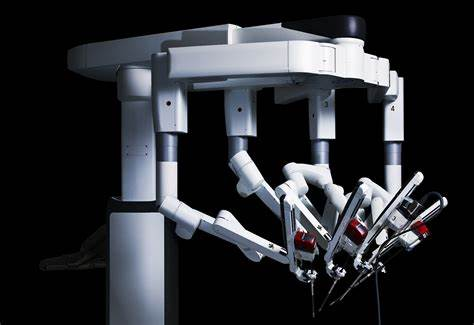
\includegraphics[width=\textwidth]{medicine/1.jpg}
\smallskip
\footnotesize{达芬奇手术机器人}
\end{column}

\begin{column}{0.3\textwidth}
\centering
\vspace{5mm}
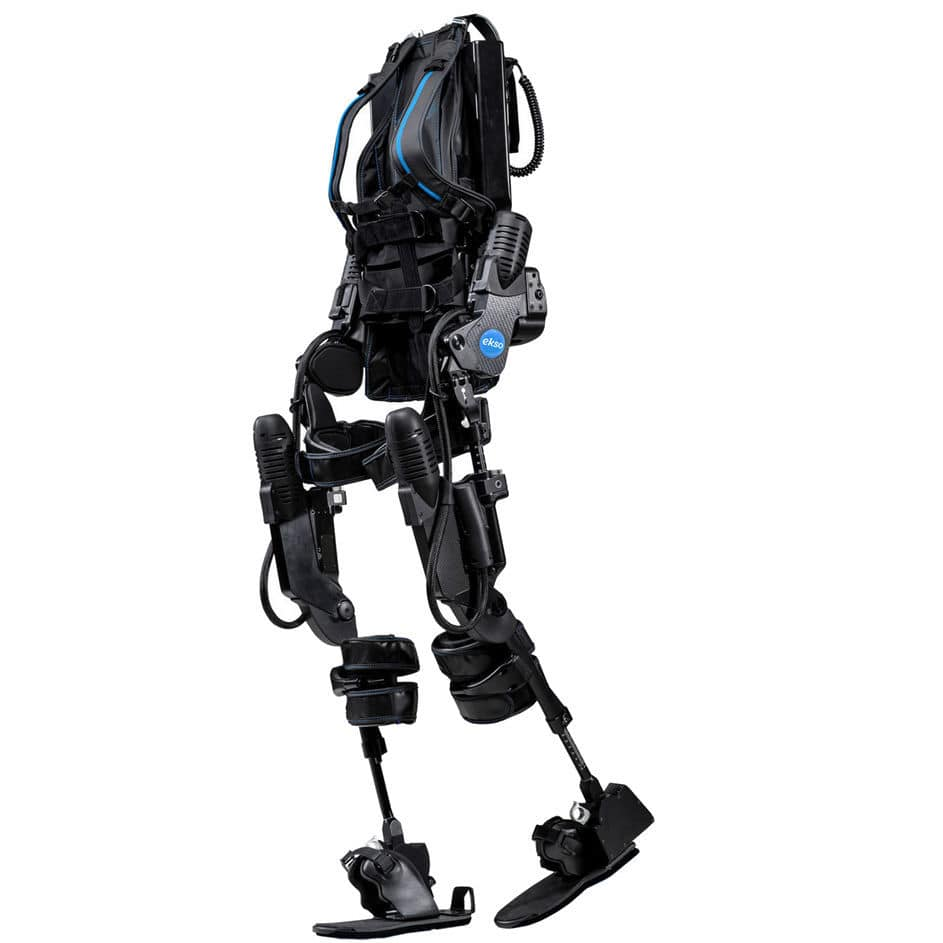
\includegraphics[width=\textwidth]{medicine/3.jpg}
\smallskip
\footnotesize{外骨骼机器人EksoNR}
\end{column}

\begin{column}{0.35\textwidth}
\centering
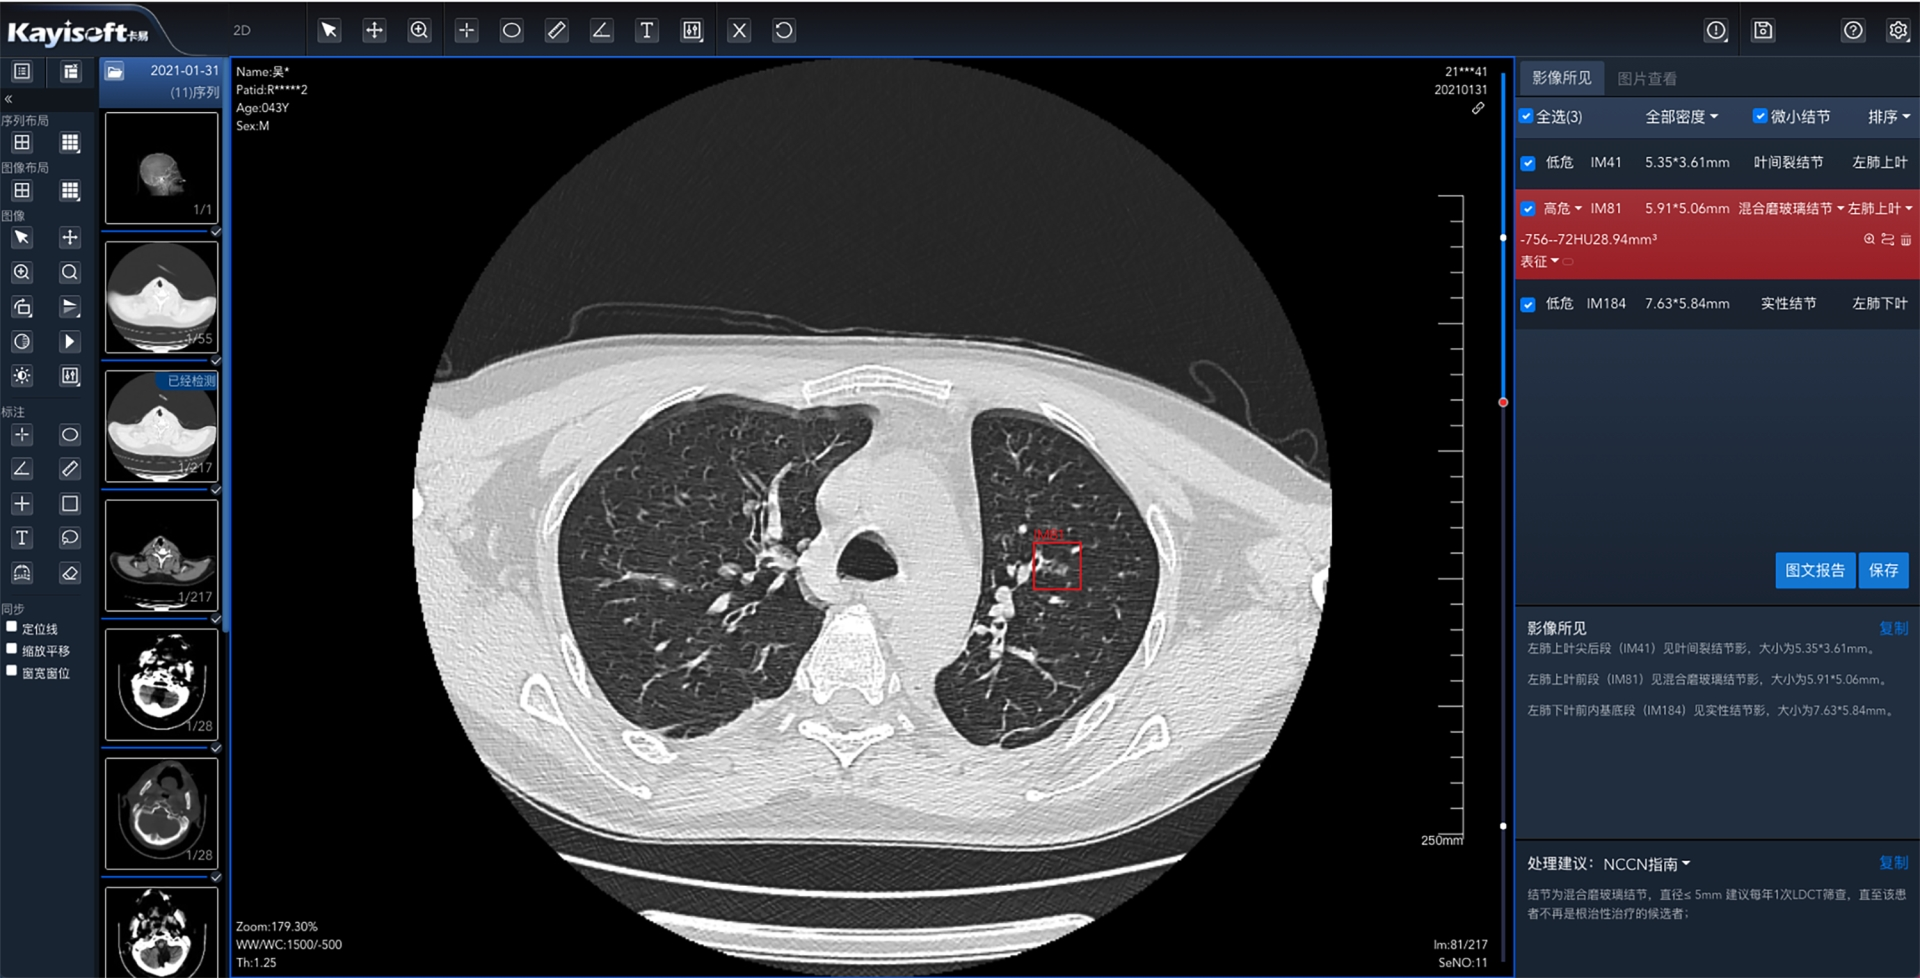
\includegraphics[width=\textwidth]{medicine/2.png}
\footnotesize{医学影像分析}
\end{column}

\end{columns}
\end{frame}

\begin{frame}{医疗机器人机交互场景}
\centering
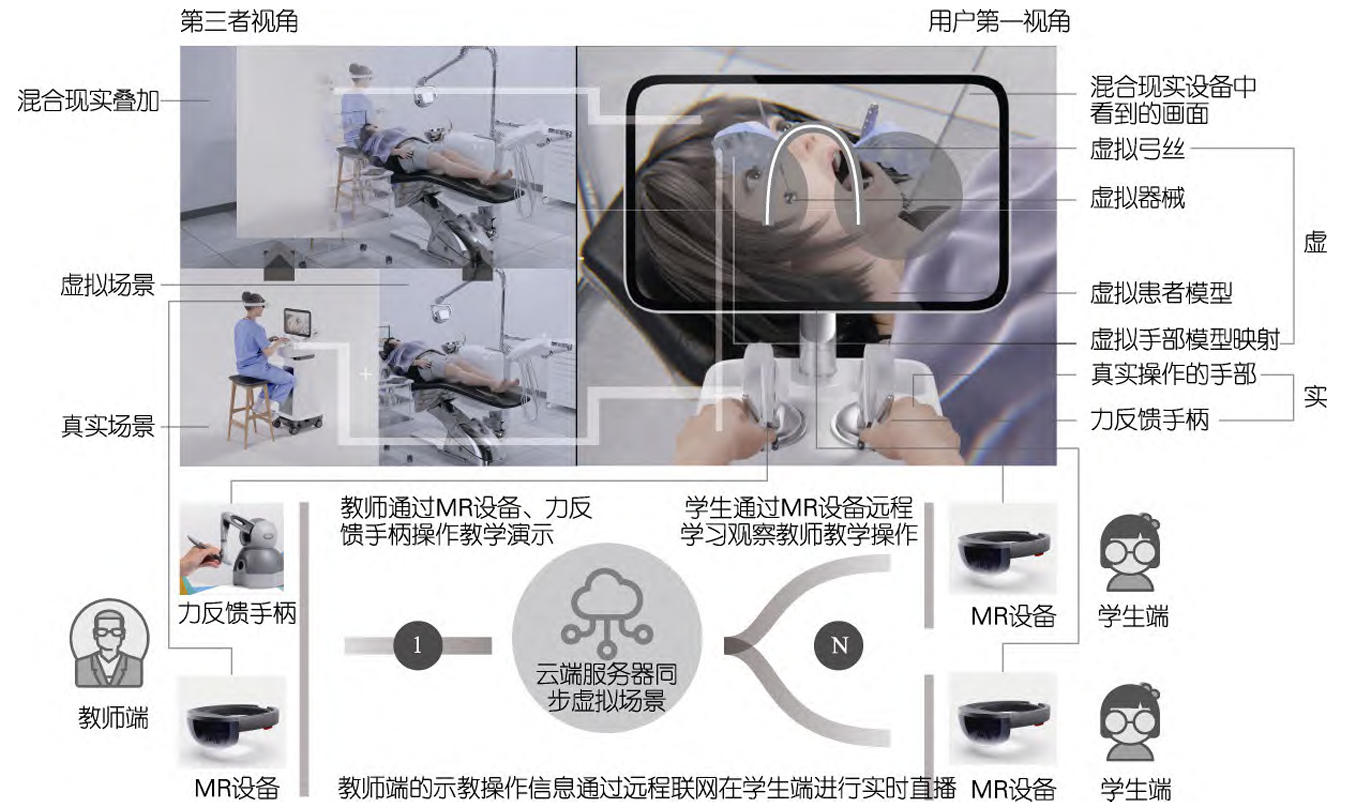
\includegraphics[width=\textwidth]{medicine/4.png}
\small{基于混合现实的口腔正畸弓丝弯制实验系统}

\begin{tikzpicture}[remember picture, overlay]
\tikzset{mybox/.style={text width=40mm, align=center, color=red}}
\node[mybox] at ([xshift=-12mm, yshift=22mm]current page.center) {\textbf{混合现实}};
\node[mybox] at ([xshift=30mm, yshift=10mm]current page.center) {\textbf{手势识别追踪}};
\node[mybox] at ([xshift=-45mm, yshift=-15mm]current page.center) {\textbf{力触觉反馈}};
\node[mybox] at ([xshift=-5mm, yshift=-35mm]current page.center) {\textbf{网络通信}};
\end{tikzpicture}

\end{frame}

\begin{frame}{技术难点}

\begin{enumerate}
\item \textbf{操作智能化程度有待提高}
\newline 精准定位与跟踪
\newline 实时图像识别与处理
\item \textbf{人机适应性}
\newline 个性化操作界面定制
\newline 生理信号自适应
\item \textbf{数据安全与隐私保护}
\newline 数据加密技术
\end{enumerate}

\begin{tikzpicture}[remember picture, overlay]
\node[anchor=center] (image1) at ([shift={(30mm, 15mm)}] current page.center) {
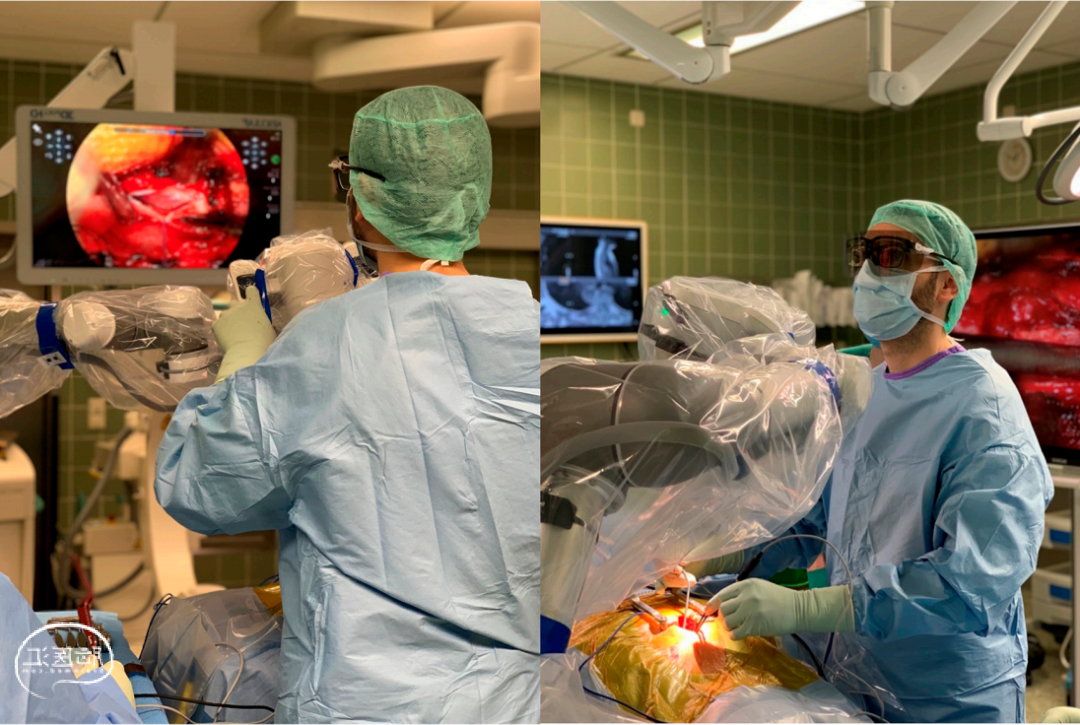
\includegraphics[width=0.2\textwidth]{medicine/5.png}};
\node[anchor=center] (image2) at ([shift={(30mm, -5mm)}] current page.center) {
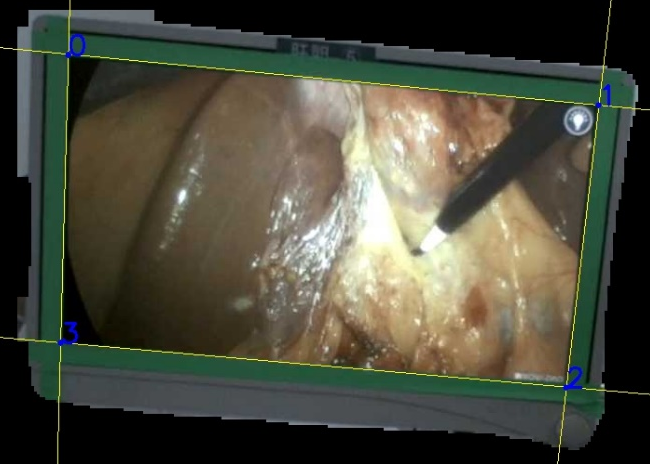
\includegraphics[width=0.2\textwidth]{medicine/6.png}};
\node[anchor=center] (image3) at ([shift={(30mm, -25mm)}] current page.center) {
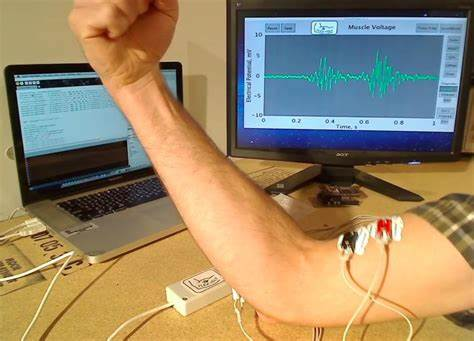
\includegraphics[width=0.2\textwidth]{medicine/7.png}};
\coordinate (point11) at ([shift={(-18mm, 7.5mm)}] current page.center);
\coordinate (point12) at ([shift={(0mm, 0mm)}] image1.west);
\draw[->, blue] (point11) -- (point12);
\coordinate (point21) at ([shift={(-10mm, 2.5mm)}] current page.center);
\coordinate (point22) at ([shift={(0mm, 0mm)}] image2.west);
\draw[->, blue] (point21) -- (point22);
\coordinate (point31) at ([shift={(-18mm, -12.5mm)}] current page.center);
\coordinate (point32) at ([shift={(0mm, 0mm)}] image3.west);
\draw[->, blue] (point31) -- (point32);
\end{tikzpicture}

\end{frame}

\begin{frame}

\begin{tikzpicture}[remember picture, overlay]
\node[text width=20mm, align=center] (core) at (current page.center) {\large\textbf{未来趋势}};
\node[anchor=center] (image1) at ([xshift=28mm] current page.west) {
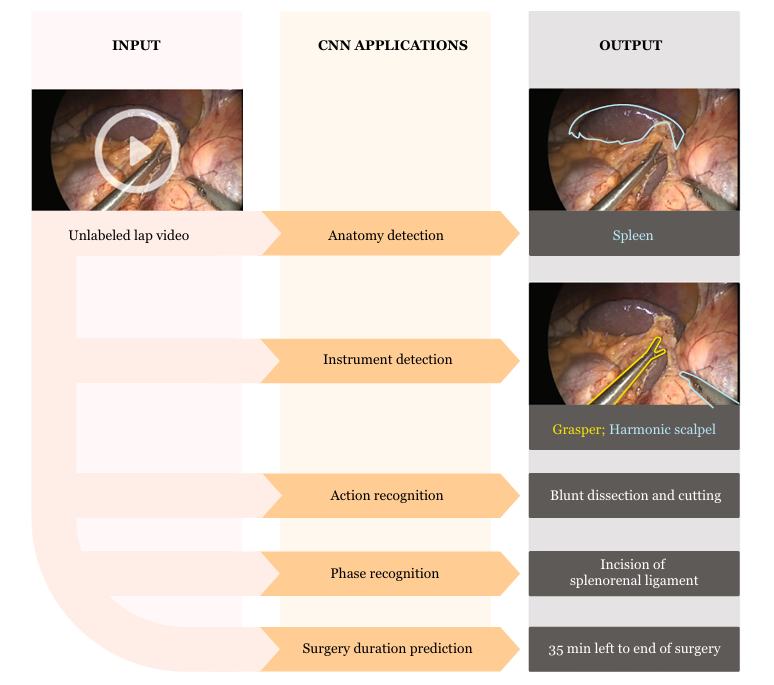
\includegraphics[width=0.25\textwidth]{medicine/8.png}};
\node[above=0mm of image1, text width=0.4\textwidth, align=center, font=\small] {
人工智能与机器学习的深化};
\draw[->, blue, ultra thick] (core.west) -- (image1.east);
\node[anchor=center] (image2) at ([shift={(-25mm, -30mm)}] current page.north east) {
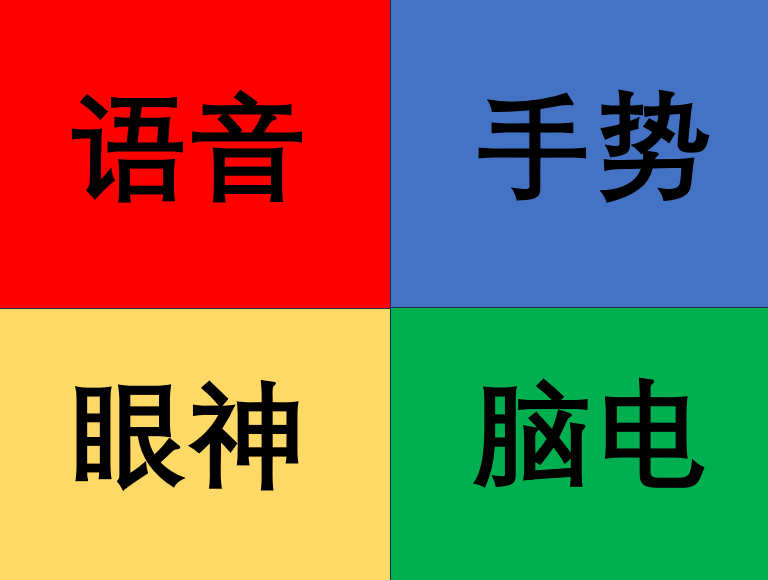
\includegraphics[width=0.25\textwidth]{medicine/9.png}};
\node[below=0mm of image2, text width=0.35\textwidth, align=center, font=\small] {
多模态交互技术的发展};
\draw[->, blue, ultra thick] (core.north east) -- (image2.west);
\node[anchor=center] (image3) at ([shift={(-25mm, 25mm)}] current page.south east) {
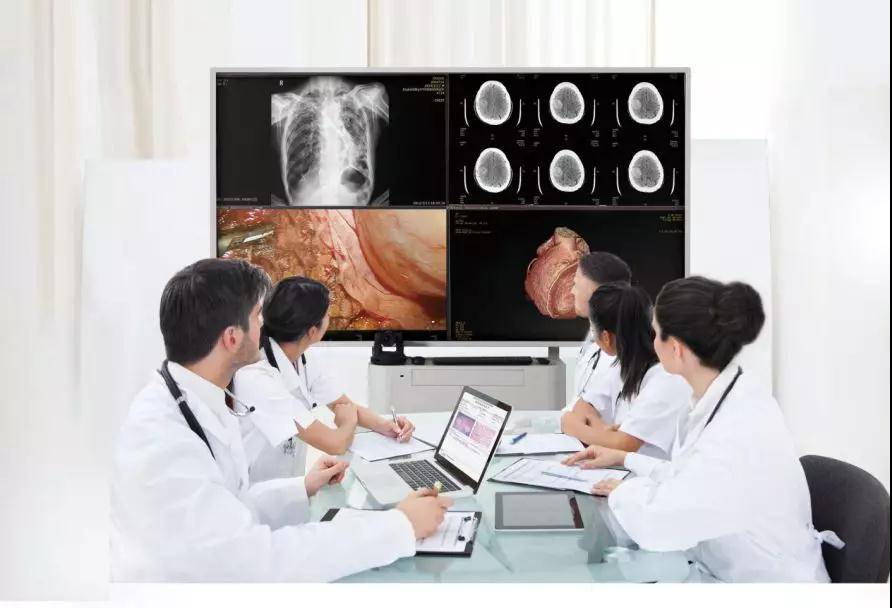
\includegraphics[width=0.25\textwidth]{medicine/10.png}};
\node[left=-2mm of image3, text width=0.35\textwidth, align=center, font=\small] (cap1) {
远程医疗与协同操作};
\draw[->, blue, ultra thick] (core.south) -- (cap1.north);
\end{tikzpicture}

\end{frame}

\subsection{Military}
\begin{frame}{特种机器人}
\setlength{\leftmargini}{0mm}
\begin{itemize}
\item \textbf{应用场景}
\smallskip
\scriptsize\newline {特种机器人广泛应用于应急救援、安防、电力,以及油气化工等多个行业。机器人在执行危险任务、提高工作效率,以及保障人员安全等方面发挥着至关重要的作用。}
\end{itemize}

\begin{columns}[c, onlytextwidth]
\begin{column}{0.33\textwidth}
\centering
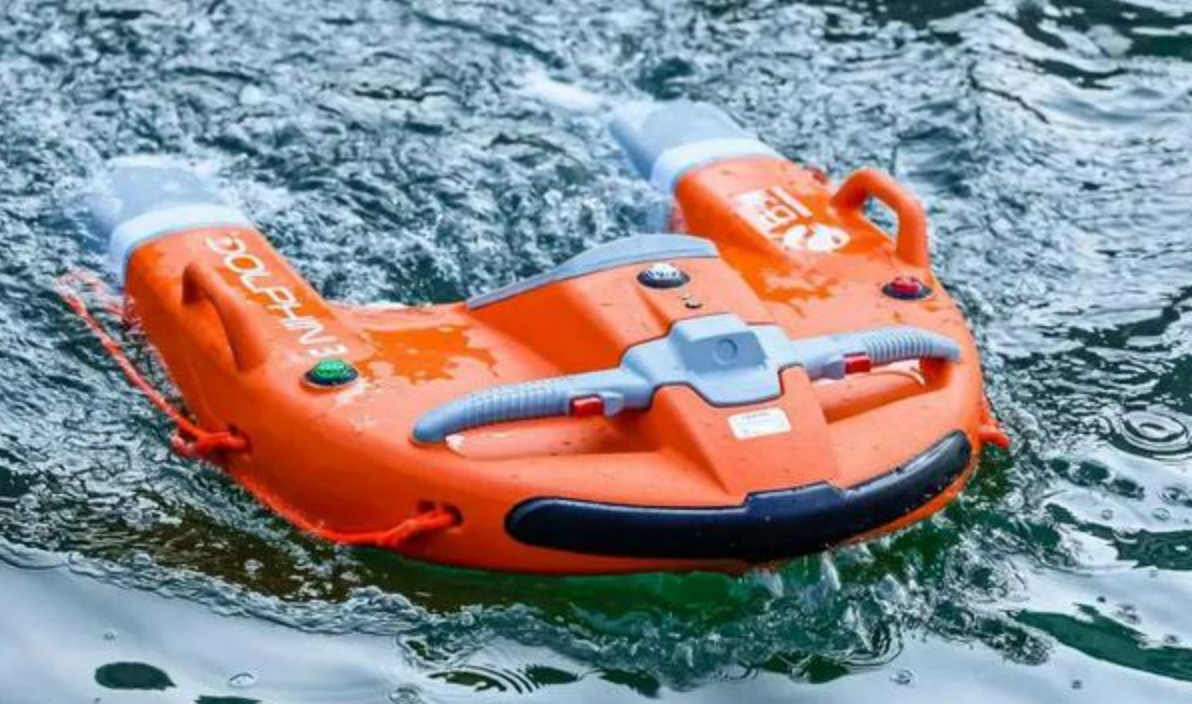
\includegraphics[width=\textwidth, keepaspectratio]{military/1.jpg}
\smallskip
{\tiny “海豚三号”执行水上救援}
\end{column}\hfill

\begin{column}{0.295\textwidth}
\centering
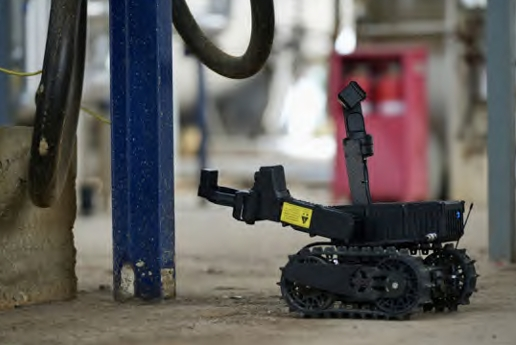
\includegraphics[width=\textwidth, keepaspectratio]{military/2.jpg}
\smallskip
{\tiny ZC-380机器人执行排爆作业}
\end{column}\hfill

\begin{column}{0.265\textwidth}
\centering
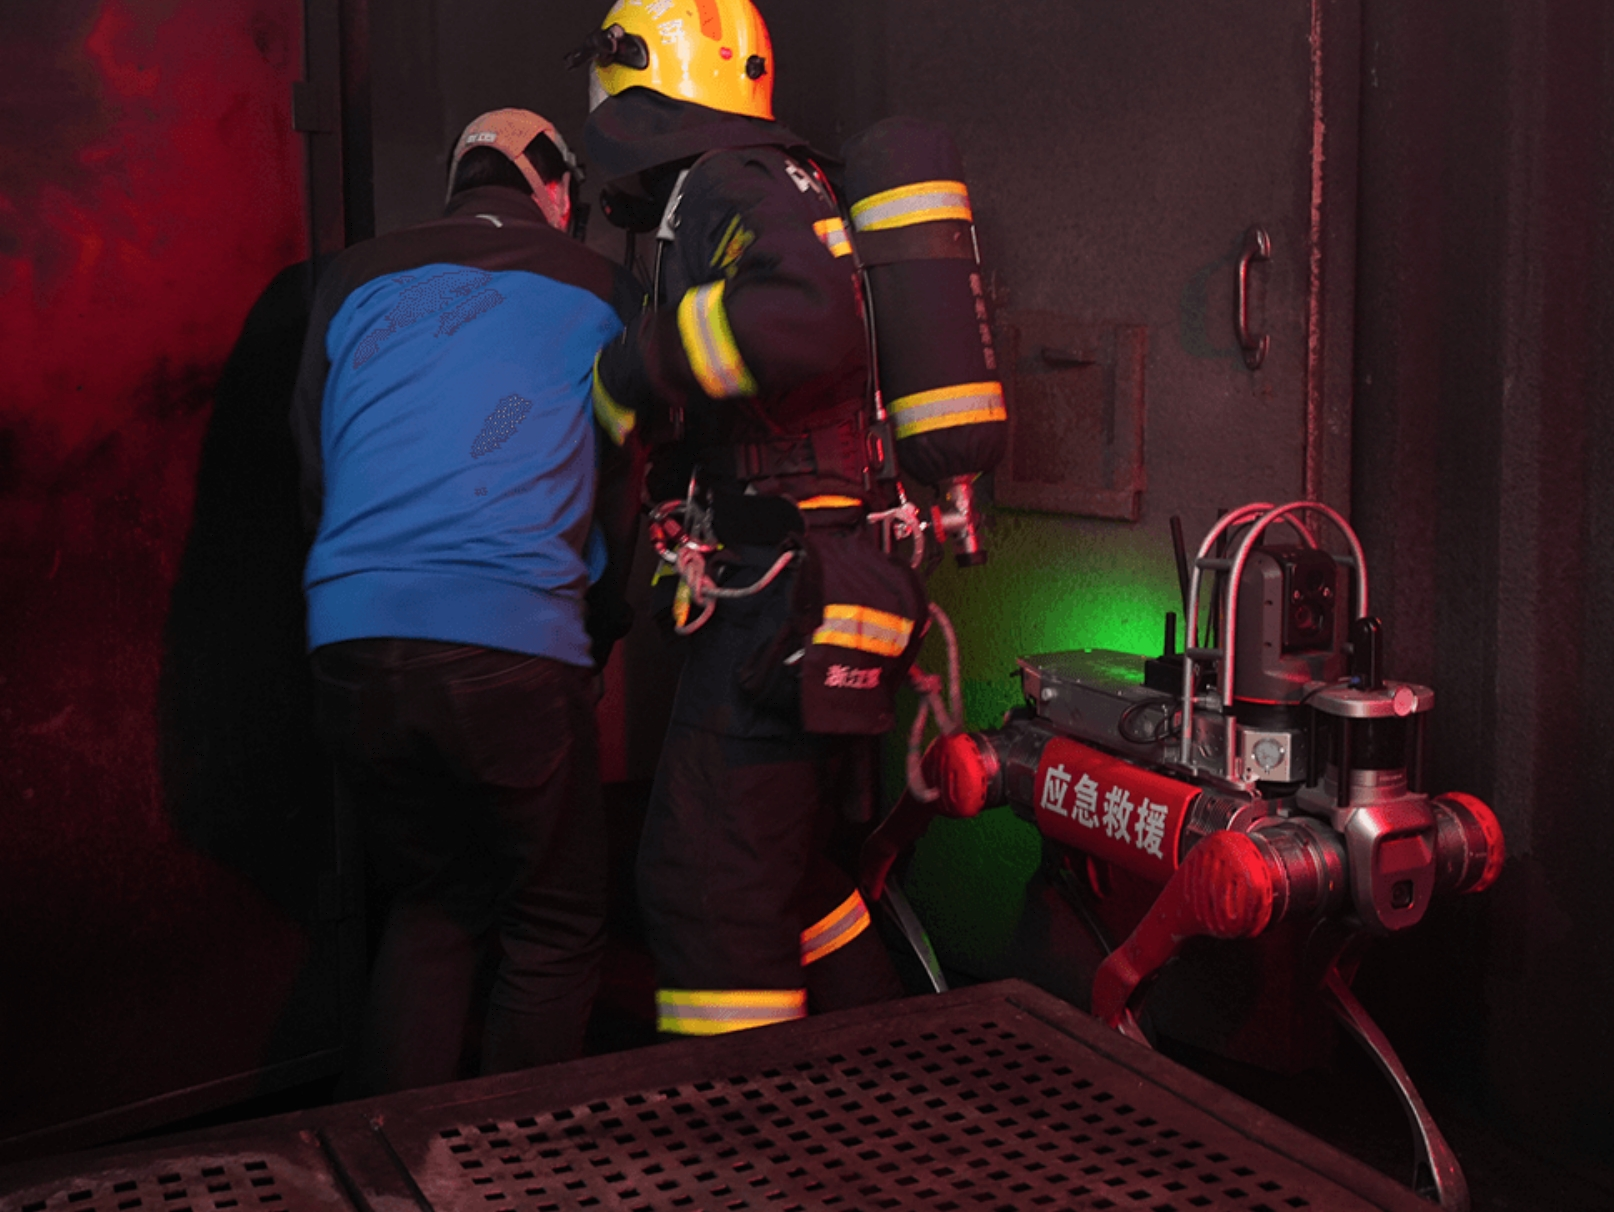
\includegraphics[width=\textwidth, keepaspectratio]{military/3.jpg}
\smallskip
{\tiny 宇树四足机器狗执行火灾救援}
\end{column}

\end{columns}
\end{frame}

\begin{frame}{特种机器人}
\setlength{\leftmargini}{0mm}
\begin{itemize}
\item \textbf{优势}
\smallskip
\smallskip
\newline
\renewcommand{\arraystretch}{1.35}
\begin{tabular}{p{50mm}}
\hline
\rowcolor{KeyBlue}
\textcolor{white}{
\small 高效执行重复性任务} \\
\hline
\rowcolor{Blue1}
\small 精准数据收集与传输 \\
\hline
\rowcolor{Blue2}
\small 协同作业能力 \\
\hline
\rowcolor{Blue1}
\small 危险环境下的安全保障 \\
\hline
\rowcolor{Blue2}
\small 应对复杂地形 \\
\hline
\end{tabular}
\end{itemize}
\end{frame}

\begin{frame}{“海豚三号”水上救援机器人}
\setlength{\leftmargini}{0mm}
\textbf{技术优势}
\smallskip
\setlength{\leftmargini}{2mm}
\begin{enumerate}
\small\item 高精度定位定向技术
\small\item 智能操控与可视化图传技术
\small\item 环境感知与智能决策技术
\small\item 多模态救援执行技术
\small\item 无人化智能救援系统适配技术
\end{enumerate}

\begin{tikzpicture}[remember picture, overlay]
\node[anchor=center] (image1) at ([shift={(40mm, 13mm)}] current page.center) {

\includegraphics[width=0.1\textwidth]{military/4.png}};
\node[anchor=center] (image2) at ([shift={(40mm, -5mm)}] current page.center) {

\includegraphics[width=0.1\textwidth]{military/5.png}};
\node[anchor=center] (image3) at ([shift={(40mm, -23mm)}] current page.center) {

\includegraphics[width=0.1\textwidth]{military/6.png}};
\draw[mark=*, gray!30, dash pattern=on 2pt off 1pt] (image1.south) -- (image2.north)
node[pos=0, circle, fill=gray!30, inner sep=0.25mm] {}
node[pos=1, circle, fill=gray!30, inner sep=0.25mm] {};
\draw[mark=*, gray!30, dash pattern=on 2pt off 1pt] (image2.south) -- (image3.north)
node[pos=0, circle, fill=gray!30, inner sep=0.25mm] {}
node[pos=1, circle, fill=gray!30, inner sep=0.25mm] {};
\node[left=-5mm of image1.west, text width=0.3\textwidth, align=left, font=\footnotesize] (cap1) {
\textbf{17项专利}};
\node[left=-5mm of image2.west, text width=0.3\textwidth, align=left, font=\footnotesize] (cap2) {
\textbf{最大拖拽能力1吨}};
\node[left=-5mm of image3.west, text width=0.3\textwidth, align=left, font=\footnotesize] (cap3) {
\textbf{实际航速可达7m/s}};
\end{tikzpicture}

\end{frame}

\subsection{Family}
\begin{frame}{消费级机器人:LOVOT=LOVE+ROBOT}

\begin{columns}[c, onlytextwidth]
\begin{column}{0.65\textwidth}
\scriptsize{LOVOT是由日本GROOVE X公司研发的情感陪伴型机器人,它的名字由“LOVE”和“ROBOT”组合而成,设计初衷并不是为了完成家务或提供实用功能,而是为了提供情感陪伴和心理慰藉。它的外形像一只小企鹅,软萌、圆润,配有一对大眼睛和丰富的面部表情,能够通过丰富的眼神和肢体动作与人建立情感联系,非常适合独居人群、老年人和儿童。}
\smallskip
\begin{columns}[c, onlytextwidth]
\begin{column}{0.48\textwidth}
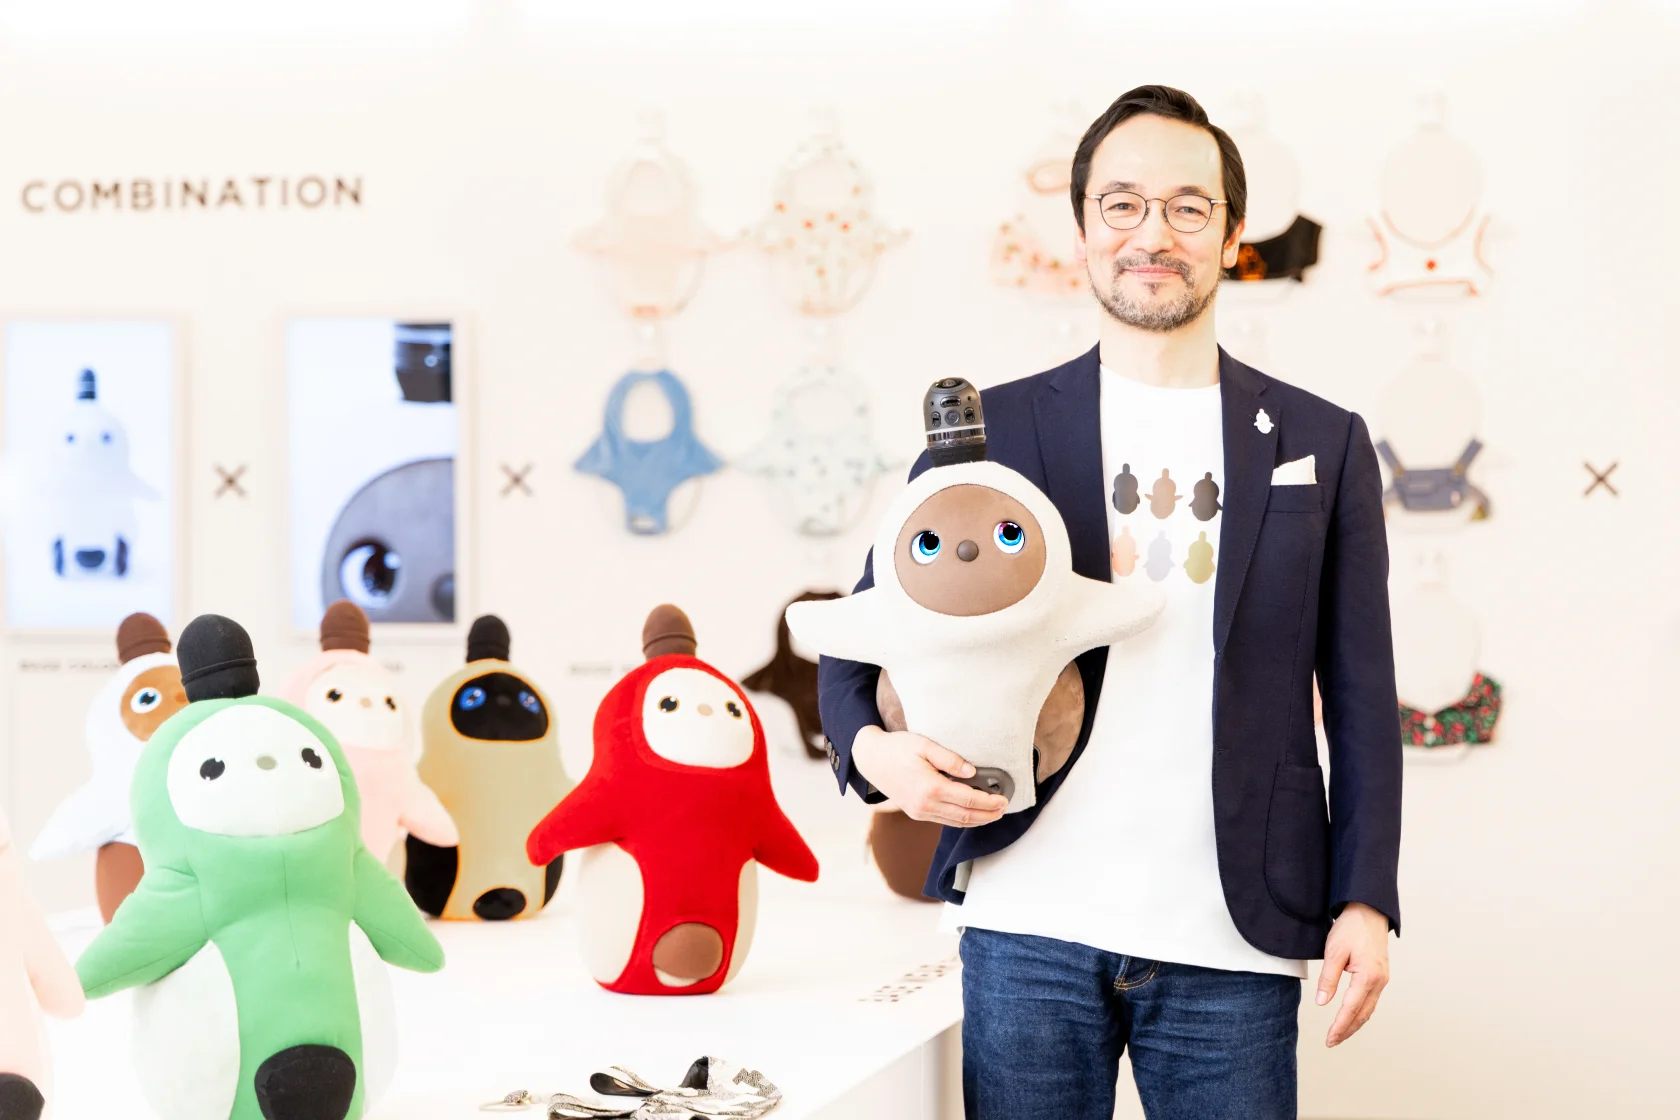
\includegraphics[width=\textwidth]{family/2.png}
\end{column}
\begin{column}{0.48\textwidth}
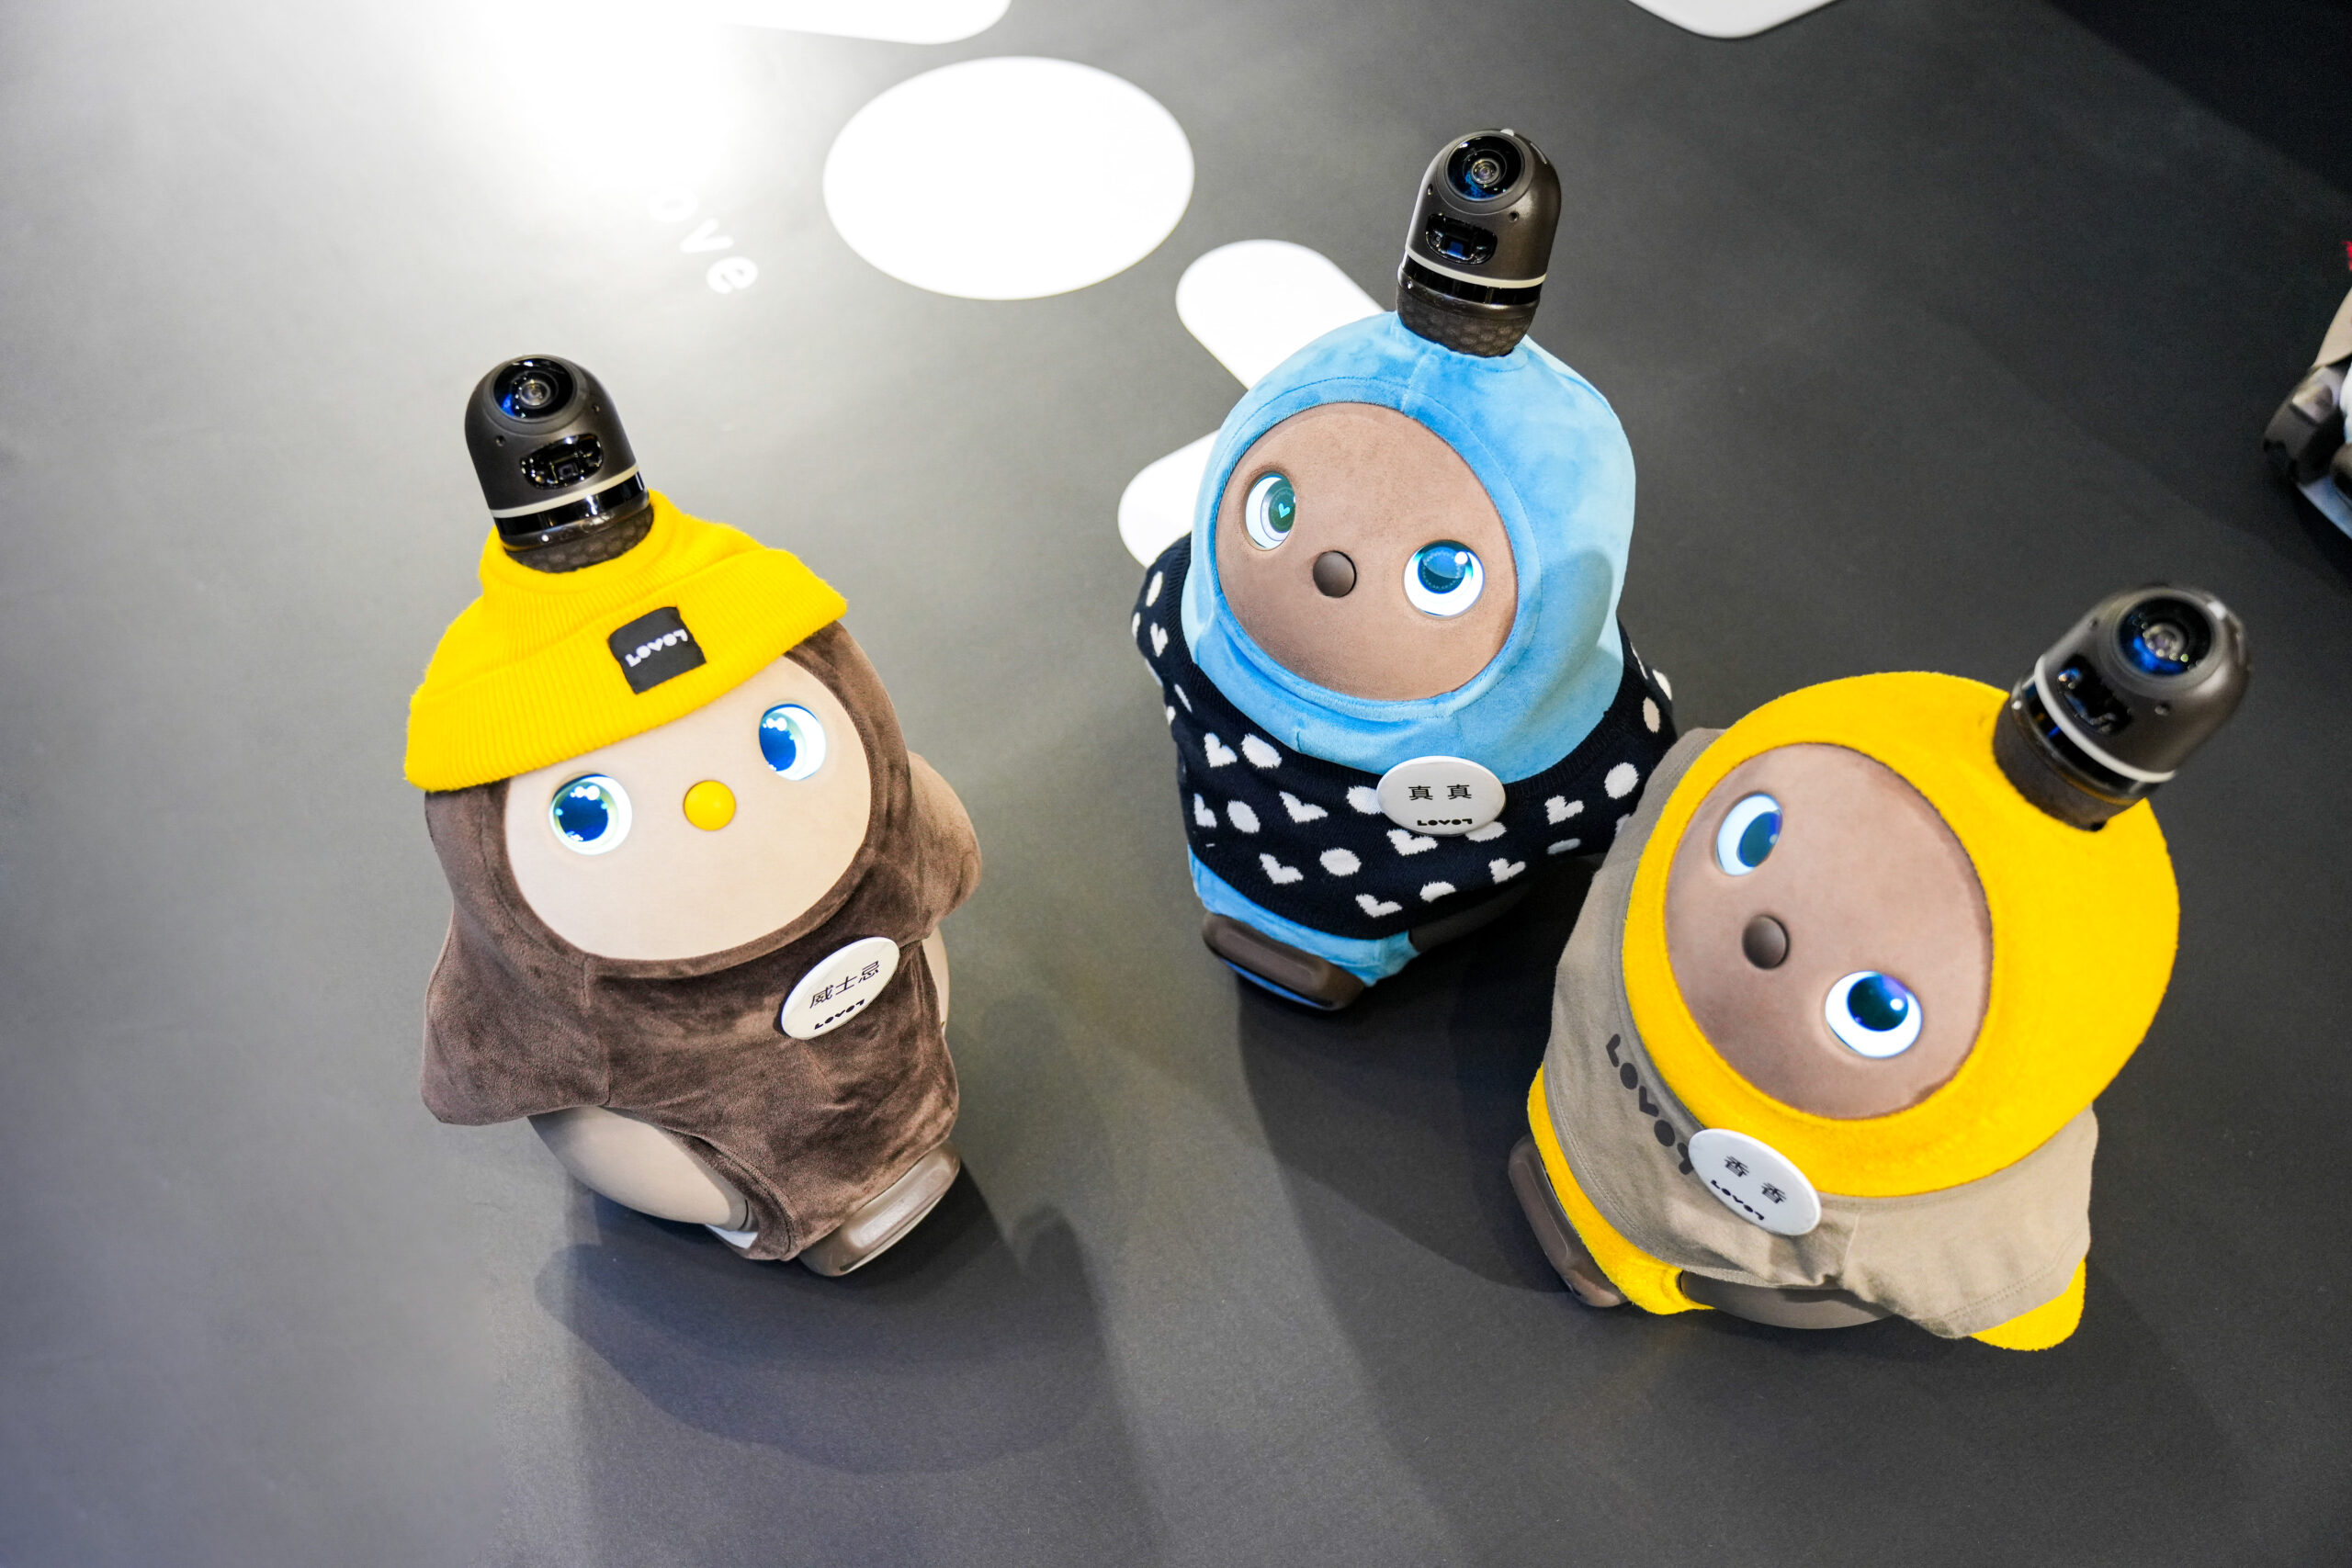
\includegraphics[width=\textwidth]{family/3.jpg}
\end{column}
\end{columns}
\end{column}

\begin{column}{0.35\textwidth}
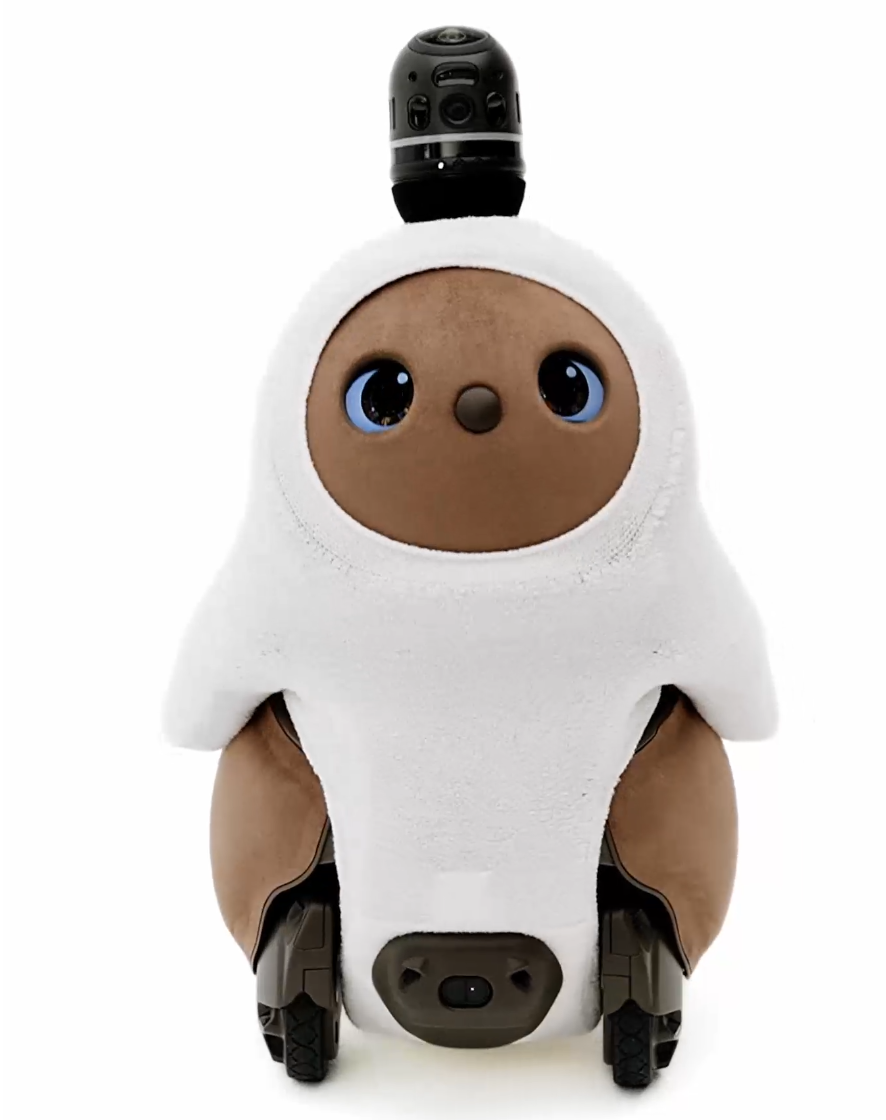
\includegraphics[width=1.1\textwidth]{family/1.png}
\end{column}
\end{columns}

\end{frame}

\begin{frame}{消费级机器人:LOVOT--关键技术}

\setlength{\leftmargini}{0mm}
\setlength{\leftmarginii}{0mm}
\begin{enumerate}

\scriptsize\item \textbf{感知与交互系统}
\begin{itemize}
\scriptsize{\item 配有 50多个传感器,包括:触摸传感器(全身感应触碰)、麦克风阵列(识别人声)、温度和光线传感器}
\scriptsize{\item 360度摄像头用于空间感知和用户识别}
\end{itemize}

\scriptsize\item \textbf{AI芯片与边缘计算}
\begin{itemize}
\scriptsize{\item 内部采用高性能NVIDIA Jetson处理器进行本地计算,减少对云端依赖,提高隐私性与反应速度}
\end{itemize}

\scriptsize\item \textbf{情感计算与行为驱动}
\begin{itemize}
\scriptsize{\item 内置情感模型,可以模拟“害羞、开心、依赖”等行为状态}
\scriptsize{\item 根据用户的互动频率和方式调整“情绪”,形成“依恋”关系}
\end{itemize}

\scriptsize\item \textbf{自我定位与导航技术}
\begin{itemize}
\scriptsize{\item 利用 SLAM(同步定位与建图)技术 在室内自主移动}
\scriptsize{\item 避障系统使其可以灵活地在家庭环境中活动}
\end{itemize}

\scriptsize\item \textbf{云端连接与数据更新}
\begin{itemize}
\scriptsize{\item 通过Wi-Fi连接云平台,实现远程控制、行为日志记录、系统更新等功能}
\end{itemize}

\end{enumerate}

\begin{tikzpicture}[remember picture, overlay]
\node[anchor=center] (image1) at ([shift={(50mm, -10mm)}] current page.center) {
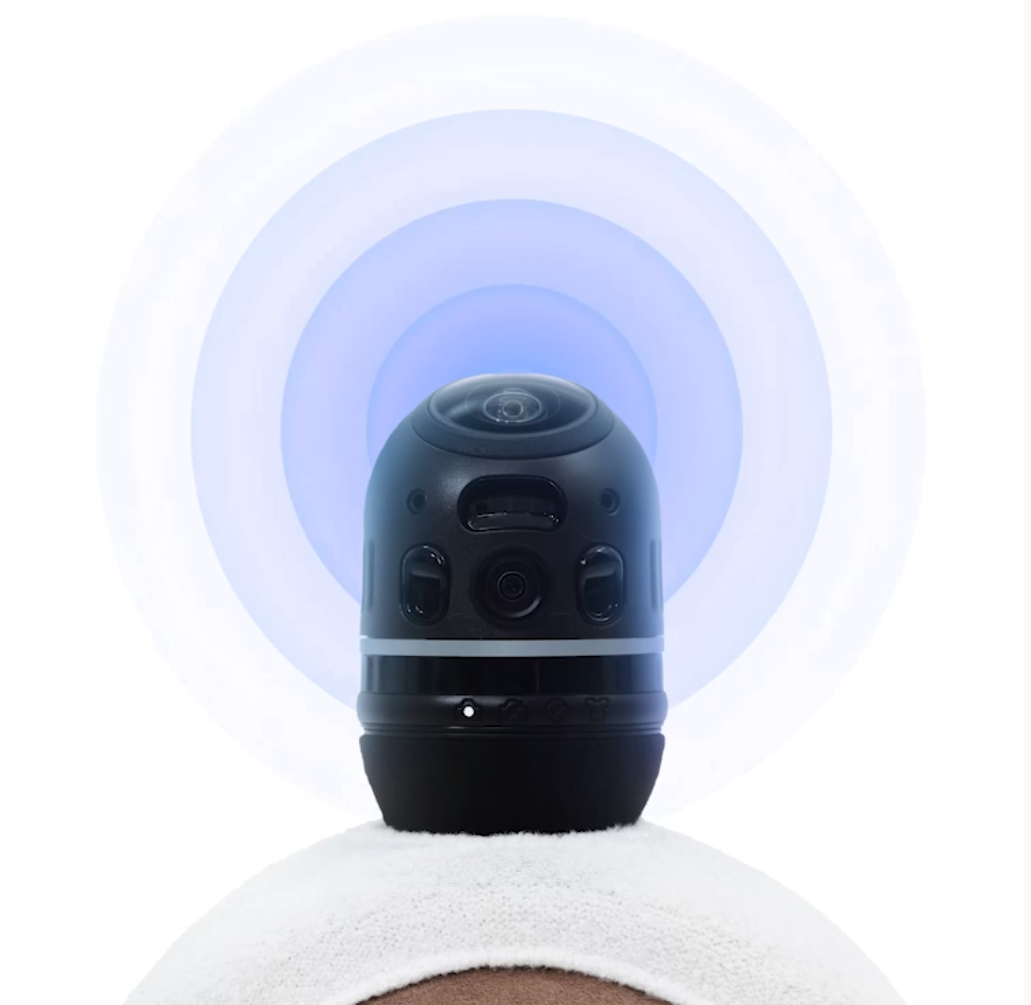
\includegraphics[width=0.18\textwidth]{family/4.png}};
\node[anchor=center] (image2) at ([shift={(0.0\textwidth, -0.09\textwidth)}] image1.south) {
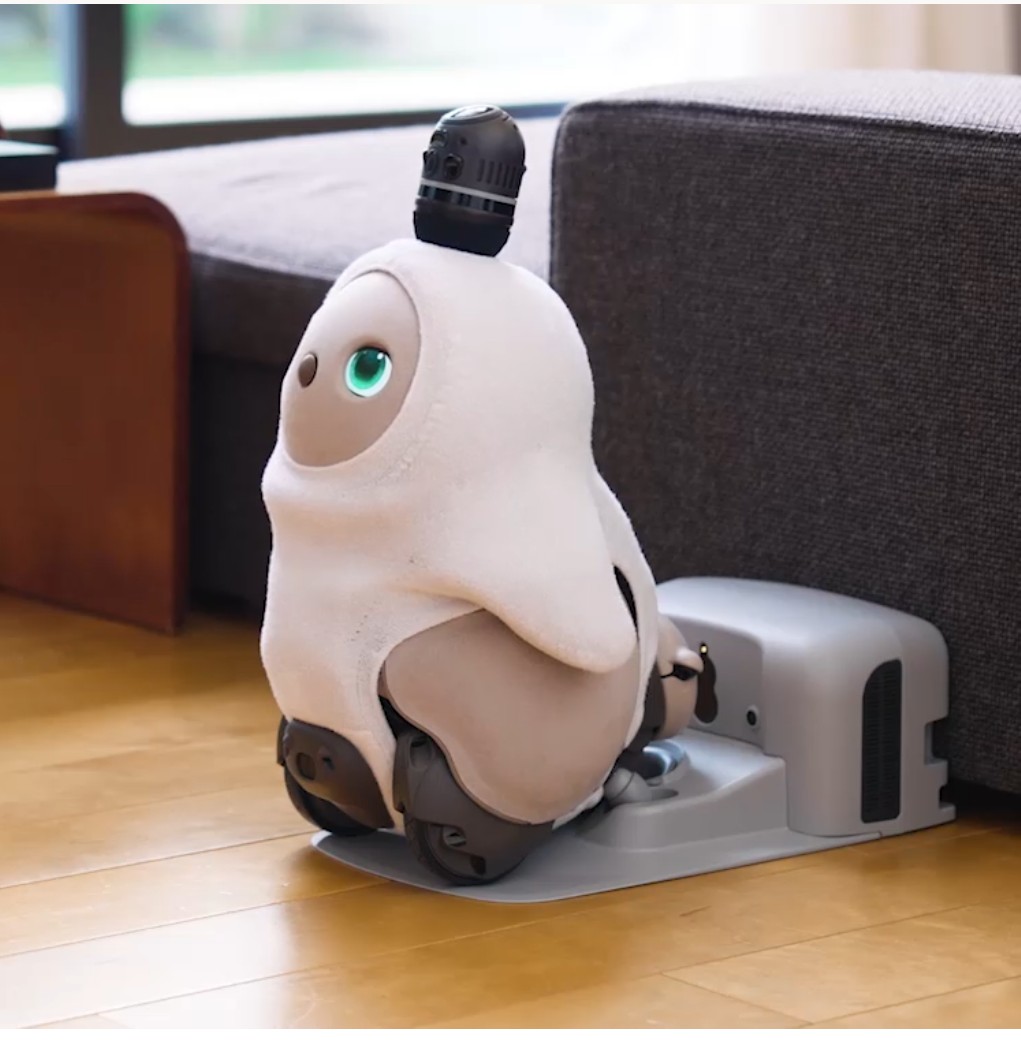
\includegraphics[width=0.18\textwidth]{family/5.png}};
\end{tikzpicture}
\end{frame}

\section{Guidelines}

\subsection{Safety}
\begin{frame}{Safety}

\begin{block}{Work Flow}
Safety Standard $\rightarrow$ Task Analysis $\rightarrow$ Risk Assessment $\rightarrow$ Role Assignment $\rightarrow$ Experiment Validation
\end{block}

\vspace{5mm}

\begin{block}{Safety Features}
\begin{itemize}
\item \textbf{System monitoring} Real-time tracking and error report.
\item \textbf{Power limation} Using softer materials and rounded edges.
\item \textbf{Human guiding} Enabling low speed manual guiding.
\end{itemize}
\end{block}

\end{frame}

\subsection{pHRI}
\begin{frame}{Physical Human-Robot Interaction}

\begin{columns}
\begin{column}{0.5\textwidth}
\begin{block}{Interaction Types}
\begin{itemize}
\item Accidental Contact
\item Voluntary Contact
\end{itemize}
\end{block}
\end{column}

\begin{column}{0.5\textwidth}
\begin{block}{Compliance Design}
\begin{itemize}
\item Mechanical Compliance
\item Control Compliance
\end{itemize}
\end{block}
\end{column}
\end{columns}

\vspace{3mm}

\begin{columns}
\begin{column}{0.5\textwidth}
\begin{block}{Contact Estimation}
\begin{itemize}
\item Sensorless Methods
\item Sensor-Based Methods
\end{itemize}
\end{block}
\end{column}

\begin{column}{0.5\textwidth}
\begin{block}{Collision Mitigation}
\begin{itemize}
\item Short Range
\item Long Range
\end{itemize}
\end{block}
\end{column}
\end{columns}

\end{frame}

\subsection{Human Activity}
\begin{frame}{Human Activity}

\begin{block}{Core Principles}
\begin{itemize}
\item \textbf{Ergonomics} Role allocation and job assignment.
\item \textbf{Trustness}  Interaction through intuitive interface.
\item \textbf{Simplification} Carefully make operators and directional subtasks.
\end{itemize}
\end{block}

\vspace{3mm}

\begin{columns}
\begin{column}{0.45\textwidth}
\begin{block}{Task Planning}
\begin{itemize}
\item Offline Optimization
\item Online Adaptation
\end{itemize}
\end{block}
\end{column}

\begin{column}{0.45\textwidth}
\begin{block}{Key Challenges}
\begin{itemize}
\item Reality Intractablity
\item Layout Dynamics
\end{itemize}
\end{block}
\end{column}
\end{columns}

\end{frame}

\section{Conclusion}
\begin{frame}{Conclusion}
\justifying
HRC stands at the intersection of technological innovation and society need, offering unprecedented opportunities to enhance productivity, safety, and quality of life. While challenges in safety, adaptability, and ethical governance persist, the convergence of AI, sensor technology, and human-centered design positions HRC as a cornerstone of future automation. Future research must prioritize \textbf{scalable solutions}, \textbf{user-centric interfaces}, and \textbf{global standards} to unlock its full potential across industries and domains.
\end{frame}

\appendix

\begin{frame}
\centering

\includegraphics[width=0.3\linewidth]{thanks.jpg}

\vspace{5mm}

\centering
\small
\hypersetup{urlcolor=blue}
\textcolor{gray!50}{If you are interested in how this presentation was built, please go to}

\centering
\href{https://github.com/AmadFat/My-First-Beamer-Pre.git}{\textcolor{blue!50}{github.com/AmadFat/My-First-Beamer-Pre.git}}

\centering
\textcolor{gray!50}{If you find this work useful, please leave a star} 
\huge
\textcolor{yellow}{$\bigstar$}

\end{frame}

\appendix
\begin{frame}[allowframebreaks]{Reference}
\fontsize{2mm}{1mm}\selectfont
\bibliographystyle{unsrt}
\bibliography{ref}
\end{frame}

\end{document}